\documentclass{article}


% if you need to pass options to natbib, use, e.g.:
    \PassOptionsToPackage{numbers, compress}{natbib}
% before loading neurips_2023


% ready for submission
% \usepackage[preprint]{neurips_2023}


% to compile a preprint version, e.g., for submission to arXiv, add add the
% [preprint] option:
    \usepackage[preprint]{neurips_2023}


% to compile a camera-ready version, add the [final] option, e.g.:
%     \usepackage[final]{neurips_2023}


% to avoid loading the natbib package, add option nonatbib:
%    \usepackage[nonatbib]{neurips_2023}


\usepackage[utf8]{inputenc} % allow utf-8 input
\usepackage[T1]{fontenc}    % use 8-bit T1 fonts
\usepackage{hyperref}       % hyperlinks
\usepackage{url}            % simple URL typesetting
\usepackage{booktabs}       % professional-quality tables
\usepackage{amsfonts}       % blackboard math symbols
\usepackage{nicefrac}       % compact symbols for 1/2, etc.
\usepackage{microtype}      % microtypography
\usepackage{xcolor}         % colors
\usepackage{natbib}
\usepackage{graphicx}
\usepackage{subcaption} % Required for subfigures


\title{A Comparative Study of CNN, ResNet, and Vision Transformers for Multi-Classification of Chest Cancerous Cells \thanks{Code and Data are available: https://github.com/Aviral-03/CSC413-Final-Project}}


% The \author macro works with any number of authors. There are two commands
% used to separate the names and addresses of multiple authors: \And and \AND.
%
% Using \And between authors leaves it to LaTeX to determine where to break the
% lines. Using \AND forces a line break at that point. So, if LaTeX puts 3 of 4
% authors names on the first line, and the last on the second line, try using
% \AND instead of \And before the third author name.

\author{
    Kaushik Murali \\
    \And
    Isha Surani \\
    \And
    Aviral Bhardwaj \\
    \And
    Ananya Jain \\
}


\begin{document}


\maketitle
\section{Introduction}

Detecting diseases early and accurately is important for the treatment and improvement of patient outcomes. Although chest X-ray imaging is a relatively low cost tool for diagnosis, the lack of access to radiologists in many areas can be a problem. Recently, there have been significant breakthroughs via the application of deep learning techniques. Among these techniques, Convolutional Neural Networks (CNNs), Residual Networks (ResNet), and Vision Transformers have proven to be important in improving the precision and efficiency of these tasks. In our project, we will conduct a comparative study of these three architectures in the multi-classification of chest cancerous cells, and then propose new solution to the existing model.

\section{Background Work}


Two prior works related to our project include: 
\begin{enumerate}
    \item \textbf{\citet{kermany2018identifying}}
This study focuses on presenting the applications of deep learning models, particularly Convolutional Neural Networks, in precisely detecting pneumonia in chest X-ray images. This study offers us insights into how CNNs can be practically applied to the medical field in the context of medical imaging. It sheds light not only the advantages but also the challenges faced when using these models for medical diagnosis.

    \item \textbf{\citet{liu2023recent}}
This research highlights how transformer models, through their attention mechanisms, are proficient at processing medical images for tasks such as disease detection, classification and segmentation. It provides a comparative analysis of the performance between the transformer-based and existing methods, and showcases how transformers may be superior to conventional methods in performing complex medical image analysis tasks in terms of accuracy and efficiency. The study not only offers us insights into how transformers have great potential in medical image analysis but also guides us in tackling obstacles we might face such as computational demands.
\end{enumerate}


\section{Data Processing}
For our project, we plan to use the publicly available dataset form the National Institues of Health (NIH) Chest X-ray dataset. This NIH Chest X-ray Dataset is comprised of 112,120 X-ray images with disease labels from 30,805 unique patients, including those relevant to cancer diagnosis.
Data-set: https://cloud.google.com/healthcare-api/docs/resources/public-datasets/nih-chest

Data Cleaning:

Initially, we will download the dataset from the NIH Chest X-ray dataset repository. We will thoroughly inspect the dataset in order to understand the structure of the dataset (image dimensions and labels) and also to identify any corrupt/missing files.
Since we are focusing on cancerous cells, we will filter the images in the dataset according to labels that would be pertinent to our project. We might have to categorize the dataset into separate classes as well if necessary.
In order to make sure that the model does not face any issues in efficiently learning from the data, we will preprocess the images through resizing to a standard size, normalization to scale pixel values and potentially augment them (scaling, rotation etc) to make the dataset diverse and ensure the model is as robust as possible.
We will split the dataset into training, testing ad validation sets. We are considering a standard split of 70\% training, 15\% testing and 15\% validation. This split makes it such that the model can be trained on a substantial quantity of data but still be appropriately validated and tested for its performance by images the model has not encountered before.

\section{Architecture}
In our project, we focus on three architectures - Convolutional Neural Networks (CNNs), Residual Networks (ResNet), and Vision Transformers. ResNets and Vision Transformers might require more computational power due to their deeper architectures and self-attention mechanisms. Please see illustration in  Section \ref{appendix} \\
 \textbf{Convolutional Neural Networks} will serve as our baseline model due to their widespread success in image recognition tasks. CNNs are perfect for medical image analysis since they are skilled at automatically identifying significant features without the requirement for manual feature extraction. The CNN architecture will be designed with multiple convolutional layers, pooling layers to reduce spatial dimensions, and fully connected layers for classification. \\
We will use \textbf{Residual Networks (ResNet)}, which use skip connections to train very deep networks, in order to solve the vanishing gradient problem that might arise with conventional deep CNNs. ResNets make it possible to train networks considerably deeper than typical CNNs by allowing activations to be passed straight to deeper layers. We will pay special attention to how well ResNet captures intricate patterns without overfitting. \\
\textbf{Vision Transformers (ViTs)} use the transformer architecture to image classification problems, marking a departure from convolution-based methods. For the model to understand the contextual links between patches, ViTs split a picture into patches and consider each patch as a token (\citet{MANZARI2023106791}). This method is useful for comprehending the spatial hierarchies found in medical imaging. 
\section{Project Plan and Ethical Consideration}

For our project, we will meet both in-person and Zoom meetings for collaborative tasks, and use WhatsApp for communication. We plan to convene weekly once we commence model implementation. We have divided ourselves into two pairs. The first pair will focus on implementing CNN and ResNet models, while the second pair will implement Vision Transformers. Following individual group work, we will convene to propose and discuss modifications to existing models. \textbf{Github} Link provided on title-page, might switch to Google Collab later. See appendix for deadline table \ref{sample-table}

Here are some of the likely risks of the project, and their corresponding solutions: \\
\textbf{Difficulty in Implementing Vision Transformer:} To mitigate this challenge, we have predetermined backup models such as DenseNet and CapsNet to ensure continuity and progress in our project. \\
\textbf{Large Dataset for Image Understanding:} We have M1 Pro/M2 with dedicated 10-cores GPU, and if needed NVIDIA 2080TI. However, if training duration exceeds expectations, we plan to consult with the (TA) to potentially reduce the dataset size or if needed we have backup datasets available. \\
\textbf{Mitigating Missing Deadlines} We have allocated "Final Checks" days within our timeline, which serve as backup days to catch up on any missed milestones, while we can have one individual who can assist both sub-groups if someone drops the course.

It is important that we consider the ethical issues of using machine learning for disease detection, and the ethical issues that come from the data collection. In a recent study, a deep learning algorithm was able to re-identify patients from anonymized medical datasets, which raises concerns about patient privacy. Biased algorithms or datasets, can lead to unintended discrimination against certain underrepresented demographic groups. Therefore it is important that we test the model is accurate and fair in real world settings with medical professionals, to ensure reliability and fairness. It would also be beneficial to not rely only on the model, but use it to help confirm diagnoses made by medical professionals.

\section{Appendix}

\label{appendix}
\begin{figure}[htbp]
  \centering
  \begin{subfigure}[b]{0.4\textwidth}
    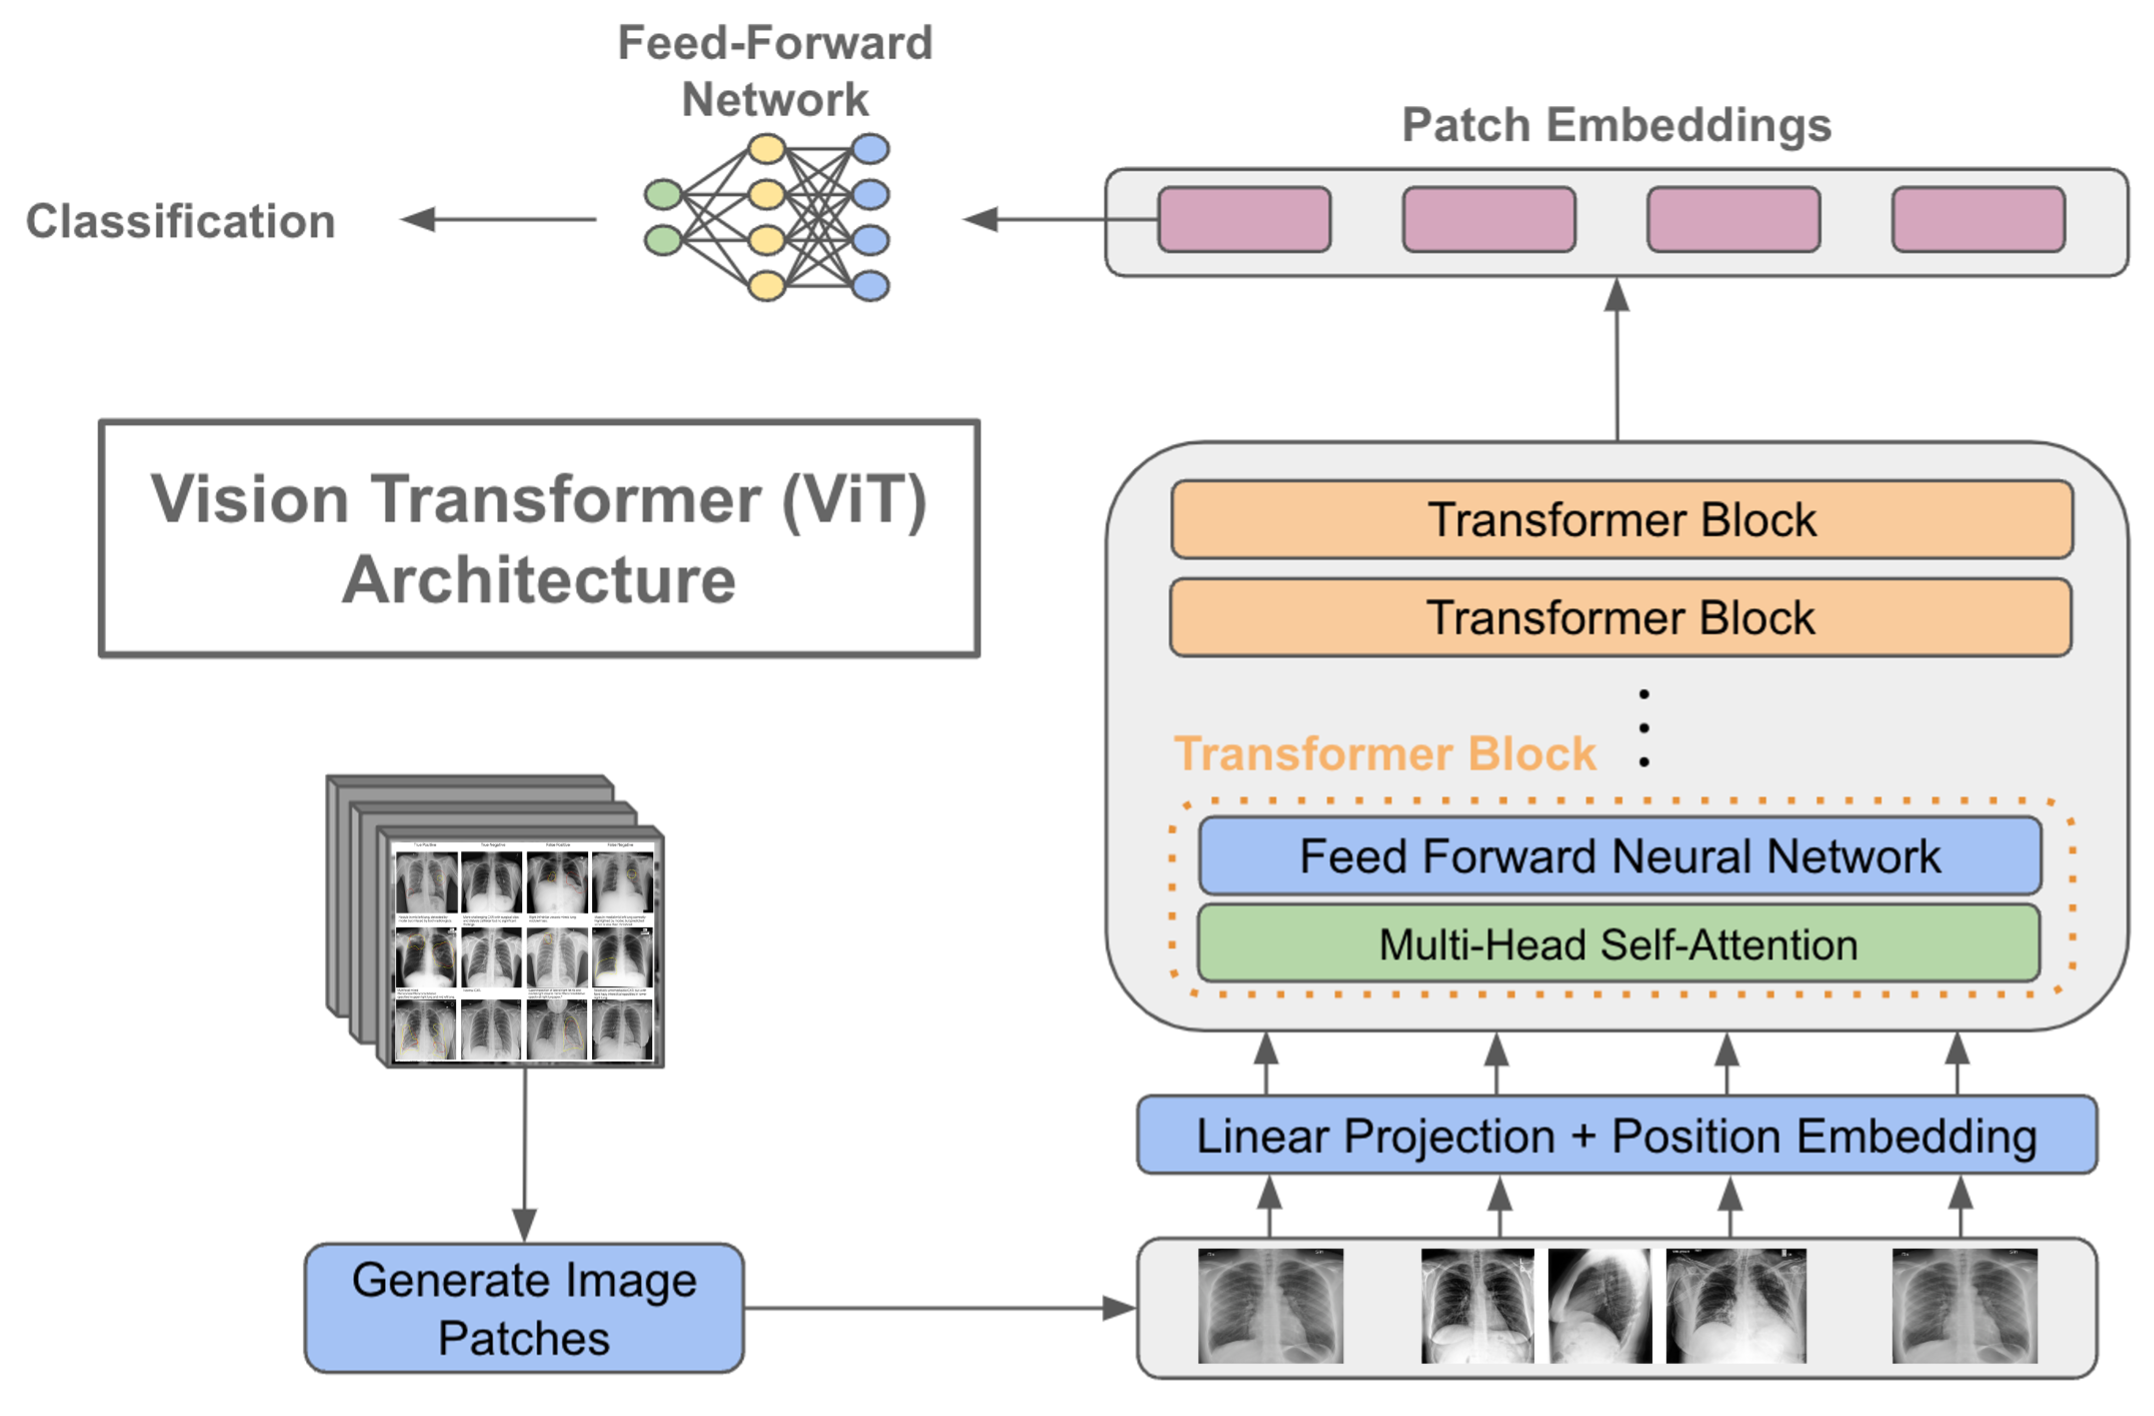
\includegraphics[width=\textwidth]{model1.png}
    \caption{Sample ViT for Chest X-Ray \cite{transformers}}
  \end{subfigure}
  \hfill
  \begin{subfigure}[b]{0.5\textwidth}
    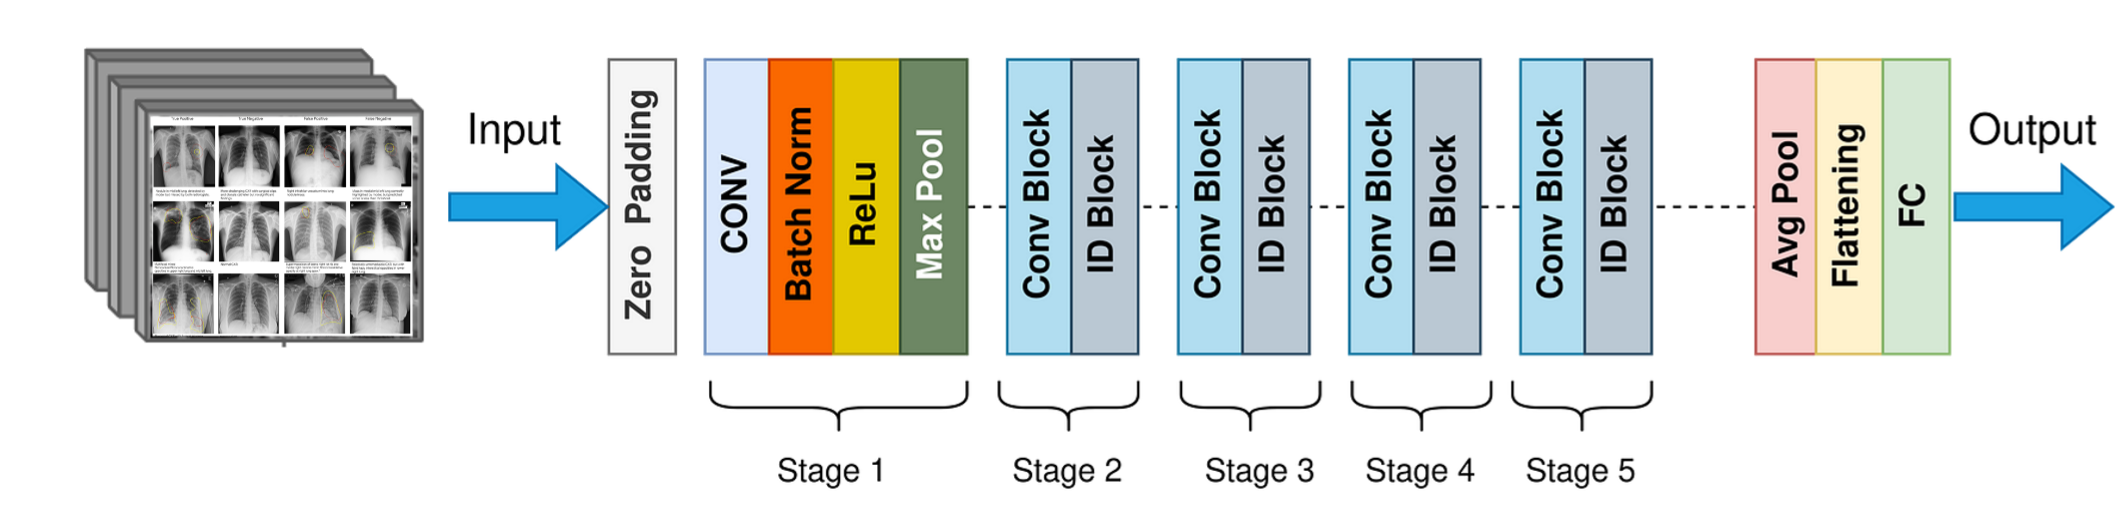
\includegraphics[width=\textwidth]{model2.png}
    \caption{ResNet50 Architecture (Sample Implementation)}
  \end{subfigure}
  \caption{ViT, and ResNet Model Illustration}
\end{figure}


\begin{table}
  \caption{Deadlines}
  \label{sample-table}
  \centering
  \begin{tabular}{lll}
    \toprule
    \cmidrule(r){1-2}
    Task     & Deadline  \\
    \midrule
    Model Implementation     & April 2nd  \\
    Research Paper Writing     & April 5th - April 15th      \\
    Final Checks & April 15th - April 19th \\
    \bottomrule
  \end{tabular}
\end{table}


\bibliographystyle{IEEEtranN}
\bibliography{references}




%%%%%%%%%%%%%%%%%%%%%%%%%%%%%%%%%%%%%%%%%%%%%%%%%%%%%%%%%%%%


\end{document}